% Capitolo 4

\chapter{Conclusioni e sviluppi futuri}
\label{Capitolo5}
\lhead{Capitolo 5. \emph{Conclusioni e sviluppi futuri}}

L'architettura e il prototipo sviluppato saranno implementati su scala
ridotta a partire dalle comunità più strutturate e che fungono già da
poli regionali, chiamati \emph{Nucleos de Formação Continuada, (NFC)},
Nuclei di Formazione Continua, che sono attualmente dieci e
geograficamente ben distribuiti sul territorio nazionale brasiliano.

Il codice prodotto consente una prima implementazione per un progetto
pilota che coinvolga sviluppatori del NPDD e consenta la formazione di
tecnici locali nei NFC, oltre ad un feedback diretto di uso da parte
delle comunità. 

Attualmente il codice supporta:
\begin{itemize}
\item autenticazione LDAP (gestione basica dei gruppi)
\item creazione e upload di contenuti audio, video e immagini
\item distribuzione tramite git-annex
\item sincronizzazione degli oggetti sui portali django (ricreando gli
  oggetti distribuiti via git-annex)
\end{itemize}

% \begin{figure}[htbp]
%   \centering
%   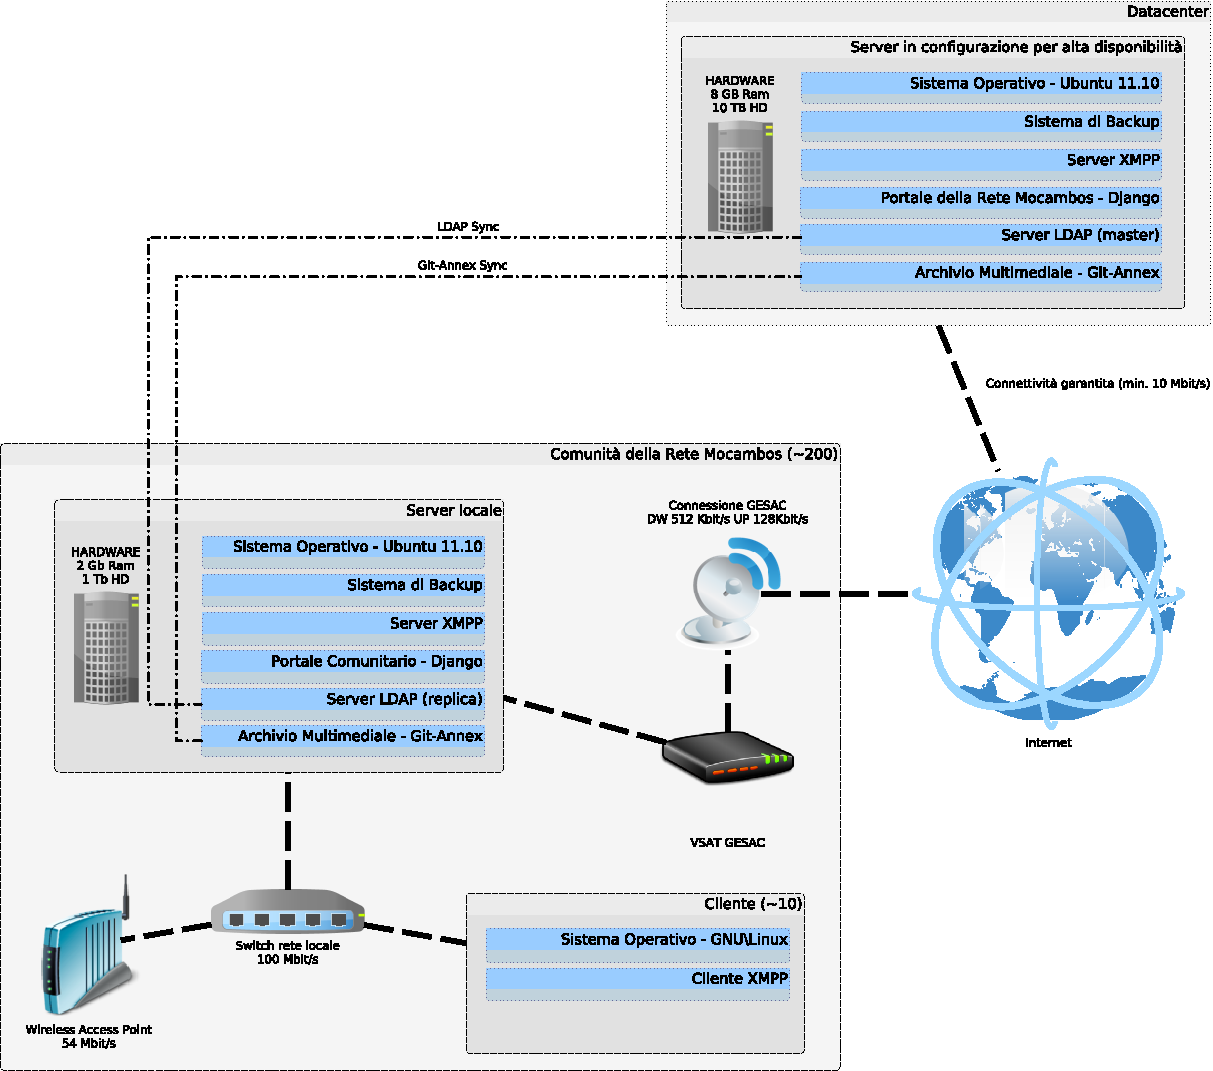
\includegraphics[width=\textwidth]{./Figure/SchemaServer_ReteMocambos-crop.pdf}
%   \rule{35em}{0.5pt}
%   \caption[Schema dell'infrastruttura della RM]{Schema dell'infrastruttura della RM.}
%   \label{fig:SchemaServer_ReteMocambos}
% \end{figure}
